\chaptr{Estado del arte}{estado-del-arte}
\sect{Aplicaciones similares}{aplicaciones-similares}

Se ha realizado una búsqueda de diferentes sitios web y aplicaciones que permitan la comunicación entre usuarios a
través de un chat en tiempo real.\ Las diferentes páginas web y aplicaciones que se han encontrado se presentan a
continuación, analizando sus características principales:

\begin{itemize}
	\item \textbf{Chateagratis.net}: Esta página web permite a los usuarios elegir un apodo (que se escoge antes de
	iniciar las conversaciones) con el que entrar en el chat, por lo que no es necesaria la creación de una cuenta de
	usuario (aunque sí que se disponga de esta funcionalidad).\ La aplicación se divide en diferentes salas, cada una
	de las cuales tiene una temática diferente y se pueden mantener multiples salas abiertas al mismo tiempo.\ Los
	usuarios pueden unirse a las salas existentes en un listado, disponible al acceder a la aplicación o en la pestaña
	asignada para ello.\ La página web permite a los usuarios enviar solamente mensajes de texto (con ciertos
	formatos, como negrita, colores, etc.) y emoticonos, sin la posibilidad de adjuntar imágenes o archivos.\ Se pueden
	programar robots para que administren una sala y que envíen mensajes automáticos cada cierto tiempo (como el que
	se visualiza en las siguientes imágenes, designado con el prefijo @).

	\begin{figure}[H]
		\centering
		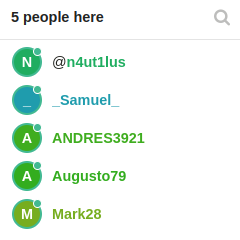
\includegraphics[scale=0.45]{ListaUsuariosChateagratis}
		\caption{Lista de usuarios conectados en una sala de chat de chateagratis.net.}
		\label{fig:ListaUsuariosChateagratis}
	\end{figure}

	\begin{figure}[H]
		\centering
		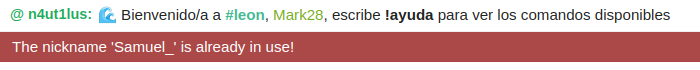
\includegraphics[scale=0.5]{ServerInfoMsgChateagratis}
		\caption{Mensajes de información del servidor en una sala de chat de chateagratis.net.}
		\label{fig:ServerInfoMsgChateagratis}
	\end{figure}

	\item \textbf{Dalechatea.me}: Esta página ofrece las mismas funciones que la anterior, pero con 2 diferencias: se
	puede modificar el tamaño del chat (ancho y alto) para adaptarlo a la pantalla y necesidades del usuario y se
	pueden mandar archivos multimedia temporales (imágenes, vídeos y audios), que se borran pasados 15 minutos.
	Además, se pueden agregar amigos, bloquear usuarios y añadir reacciones a mensajes de otros usuarios (como mandar
	un saludo o añadir a marcadores), entre otras funciones.

	\begin{figure}[H]
		\centering
		\raisebox{-0.4\height}{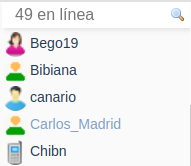
\includegraphics[scale=0.6]{ListaUsuariosDalechatea}}
		\hspace{1.5cm}
		
\includegraphics[scale=0.6]{InfoDalechatea}
		\caption{Lista de usuarios conectados y mensaje de información en una sala de chat de dalechatea.net.}
		\label{fig:UsuariosEInfoDalechatea}
	\end{figure}

\end{itemize}
\label{itm:estadoDelArte}

Ambas páginas tienen un diseño similar, con el chat en la parte central de la pantalla y un listado de usuarios en
la parte derecha (ver imagen~\ref{fig:chatCompleto}).\ La página web de chateagratis.net tiene un diseño más sencillo
y minimalista, mientras que la de
dalechatea.me tiene un diseño más moderno y con más funcionalidades.\ Ambos tienen un sistema de notificaciones y
mensajes de información, que se envían por parte del servidor del chat, para informar a todos los usuarios conectados
al mismo.\ Cuando se hace clic en un usuario, se muestra, en la parte derecha de la lista de usuarios, una ventana de
información del usuario seleccionado, que muestra su nombre de usuario y ciertos botones para realizar las acciones
previamente mencionadas.

% Además, en la parte inferior de la ventana de información del usuario se muestra un listado de los últimos mensajes
% enviados por el usuario seleccionado.
% Chats a los que pertenece el usuario.

\begin{figure}[H]
	\centering
	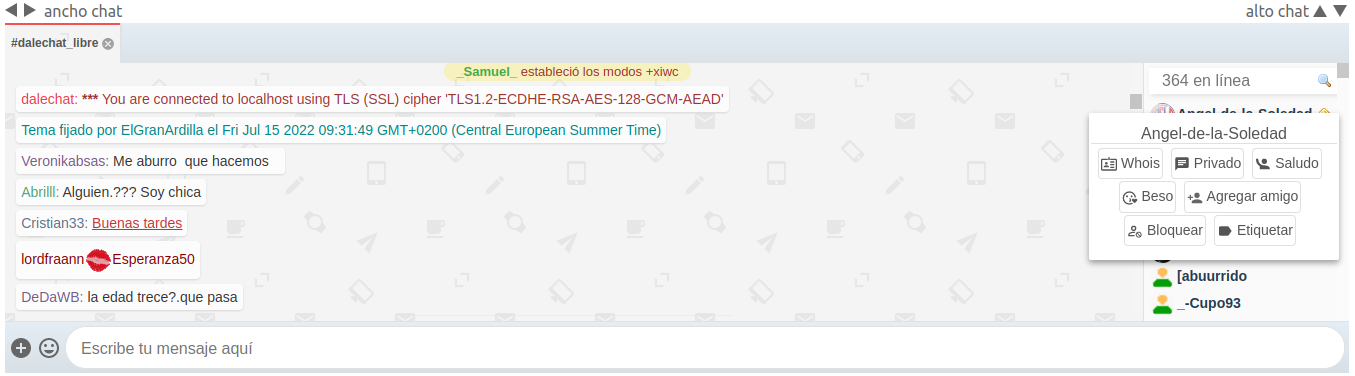
\includegraphics[scale=0.32]{Dalechatea}
	\caption{Chat completo de la página web de dalechatea.me.}
	\label{fig:chatCompleto}
\end{figure}


\sect{Opinión sobre el estado del arte}{opinion-sobre-el-estado-del-arte}
